\documentclass[11pt]{article}
\usepackage[margin=1in]{geometry}
\usepackage{graphicx}
\usepackage{booktabs}
\usepackage{amsmath}
\usepackage{hyperref}
\usepackage{xcolor}
\usepackage{float}

\title{\textbf{KV Self-Compaction Phase 2: Scaling to Qwen3-0.6B} \\[0.3em]
\large Interim Report — Phase 2a Results \& Scale-Up Status}
\author{Siddharth Agarwal \and Claude Opus 4.6}
\date{March 27, 2026}

\begin{document}
\maketitle

\begin{abstract}
We scale KV Self-Compaction from a 50M-parameter GPT model (Phase 1) to Qwen3-0.6B-Base
with LoRA finetuning on the Dolci SFT mixture. The method processes sequences in
128-token blocks, appending 16 learned compaction tokens per block whose KV states carry
compressed history to the next block. A learnable per-head attention bias (16 parameters)
controls how much the model attends to this compressed state. In Phase 2a (200 steps,
5K examples), learned compaction (Condition B) achieves cross-block perplexity of 8.44,
a 45\% improvement over random compact\_kv (Condition D, 15.26). The attention bias
diverges: B opens attention to compact\_kv ($-0.93$) while D suppresses it ($-2.13$),
confirming the model differentiates between learned and random state. Scale-up
experiments (600 steps, 50K examples, 4-GPU DDP, total batch size 512) are currently
running across 6 compute nodes (24 GPUs).
\end{abstract}

\section{Background}

KV Self-Compaction converts a pretrained transformer into a blockwise RNN with
constant-memory inference:
\begin{enumerate}
    \item Process text in blocks of $W$ tokens
    \item Append $P$ learned compaction embeddings after each block
    \item Forward the block through the transformer with a custom 4D attention mask
    \item Extract KV cache at compaction positions $\rightarrow$ \texttt{compact\_kv}
    \item Prepend \texttt{compact\_kv} to the next block's attention
    \item Train end-to-end with next-token prediction (BPTT every $K$ blocks)
\end{enumerate}

Phase 1 validated this on a 50M-param GPT model, finding that a learnable per-head
attention bias (initialized to $-2.0$) is critical for P$>$1 compaction. Without it,
softmax dilution over compact\_kv positions overwhelms predictions.

\section{Method}

\subsection{Architecture \& Training}
\begin{itemize}
    \item \textbf{Base model}: Qwen3-0.6B-Base (28 layers, 16 Q / 8 KV heads, head\_dim=128)
    \item \textbf{Adaptation}: LoRA rank=32, $\alpha$=64, targeting all 7 linear layers per block (3.28\% trainable)
    \item \textbf{Compaction}: $W$=128, $P$=16, $K$=2 (chosen via sequence length analysis of Dolci data)
    \item \textbf{New parameters}: compaction\_embeddings ($P \times 1024$) + compact\_attn\_bias ($16$ scalars)
    \item \textbf{Data}: Dolci Think-SFT + Instruct-SFT (1:1 mix), chat template with label masking
    \item \textbf{Labels}: Pre-shifted for next-token prediction (\texttt{labels[i] = token\_ids[i+1]})
\end{itemize}

\subsection{Experimental Conditions}
\begin{table}[H]
\centering
\begin{tabular}{clp{8cm}}
\toprule
Condition & Name & Description \\
\midrule
A & Full context & Standard HF forward on full sequence (no blockwise) \\
B & \textbf{Learned compaction} & Blockwise with learned compact\_kv (our method) \\
C & Truncation & Standard HF forward on last $W$=128 tokens only \\
D & Random compact\_kv & Same blockwise loop as B, but compact\_kv is random noise \\
E & No compact\_kv & Same blockwise loop as B, but no compact\_kv between blocks \\
\bottomrule
\end{tabular}
\caption{Experimental conditions. B vs D is the fairest comparison (both use identical blockwise training); B vs E isolates compact\_kv's contribution.}
\end{table}

\section{Phase 2a Results (200 steps, 5K examples)}

\subsection{Training Dynamics}

\begin{figure}[H]
\centering
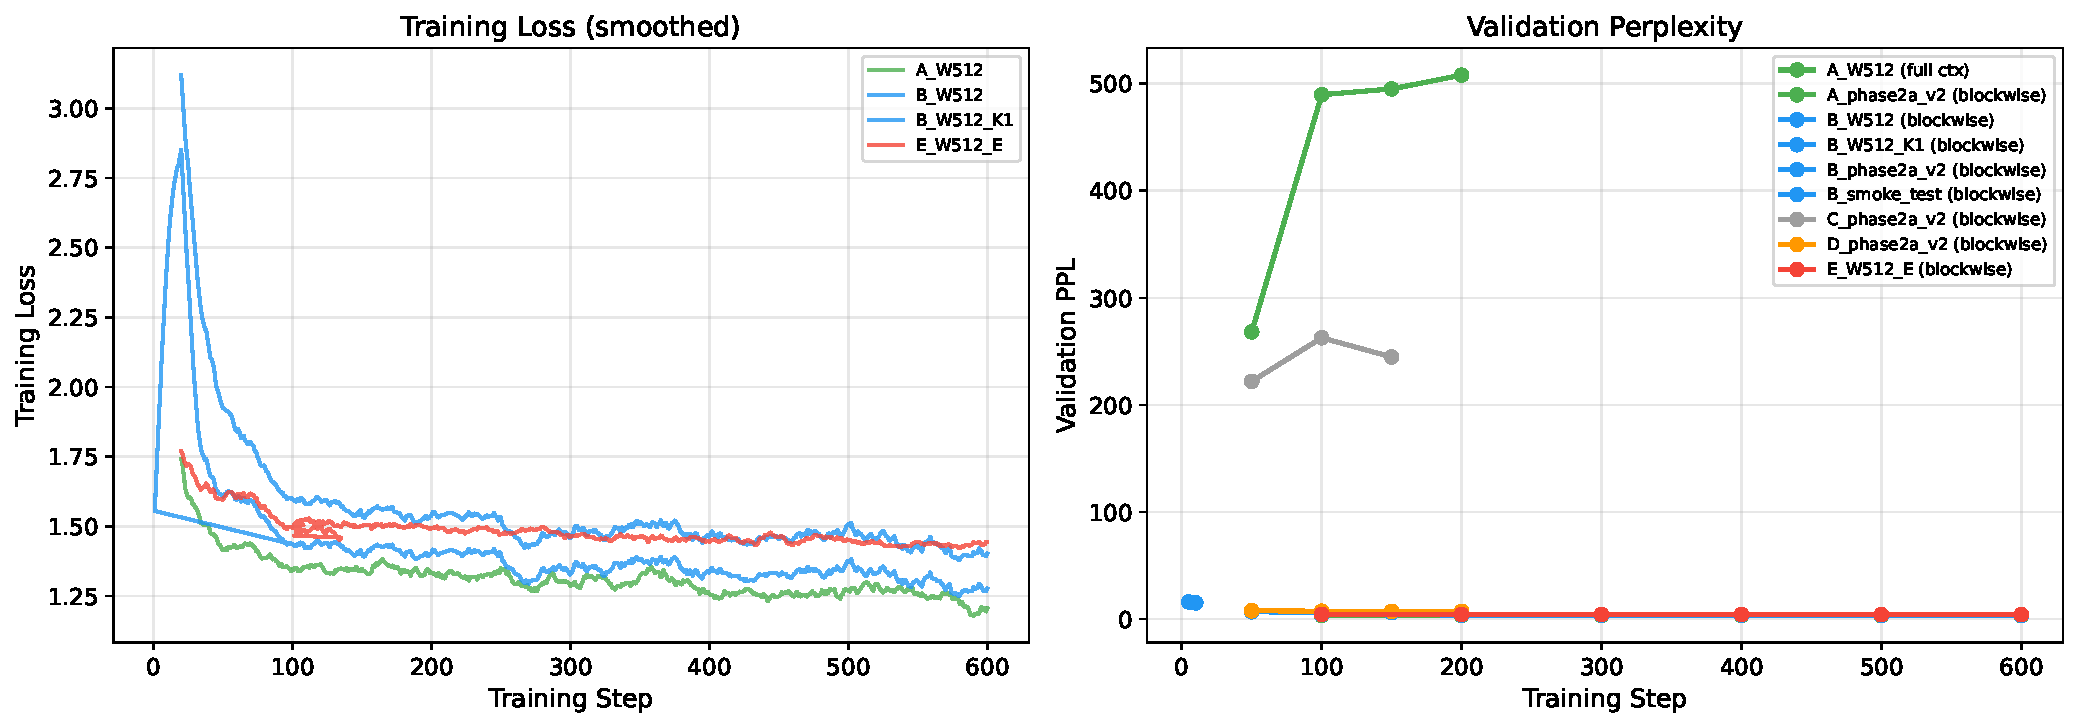
\includegraphics[width=\textwidth]{fig1_training.pdf}
\caption{\textbf{Left}: Training loss curves for all four conditions.
B and D have similar loss ($\sim$2.0), confirming both use the same blockwise mechanism.
A and C have higher loss due to different training regimes (full context and truncation respectively).
\textbf{Right}: Attention bias trajectory. B's bias moves from $-2.0$ to $-0.93$
(increasing attention to compact\_kv), while D's moves to $-2.13$ (further suppressing
random noise). This divergence is the key mechanistic evidence.}
\end{figure}

\subsection{Evaluation Metrics}

\begin{figure}[H]
\centering
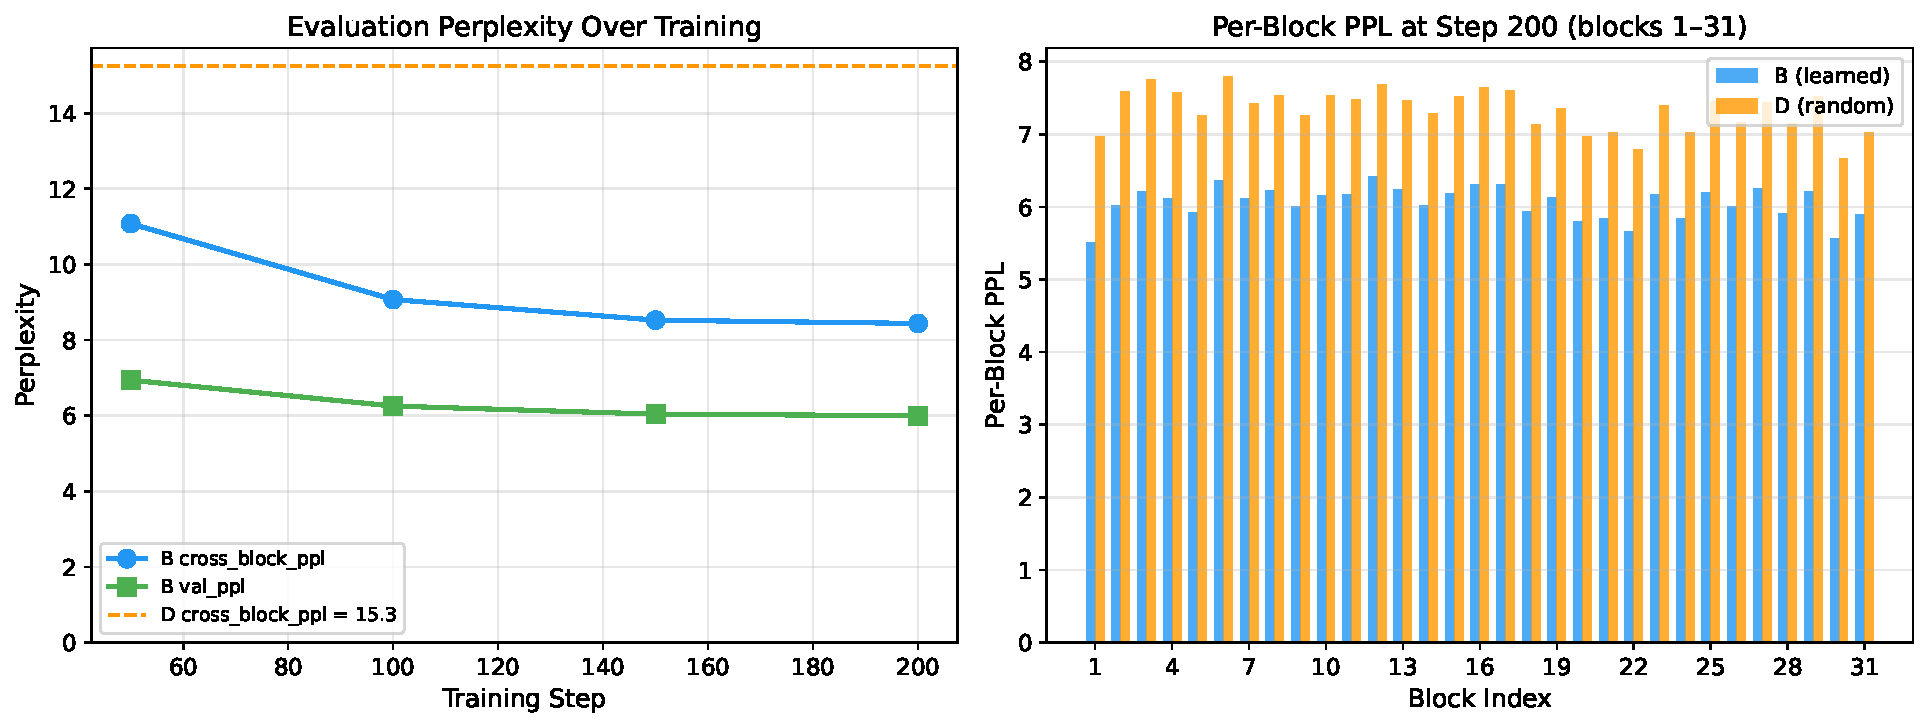
\includegraphics[width=\textwidth]{fig2_eval.pdf}
\caption{\textbf{Left}: B's cross-block and validation PPL decrease over training,
converging below D's final cross-block PPL of 15.3.
\textbf{Right}: Per-block PPL at step 200 (blocks 1--31). B consistently outperforms D
across all block positions, with remarkably uniform PPL ($\sim$5.5--6.4 for B vs $\sim$6.7--7.8 for D).}
\end{figure}

\begin{table}[H]
\centering
\begin{tabular}{lrrrr}
\toprule
Condition & val\_ppl & cross\_block\_ppl & bias\_mean & Notes \\
\midrule
\textbf{B (learned)} & \textbf{6.00} & \textbf{8.44} & $-0.93$ & Attends to compact\_kv \\
D (random kv) & 7.27 & 15.26 & $-2.13$ & Suppresses noise \\
C (truncation) & $\sim$245 & $\sim$1405 & $-2.00$ & Only 128 tokens context \\
A (full context) & 508 & 3444 & $-2.00$ & Train/eval mismatch \\
\bottomrule
\end{tabular}
\caption{Phase 2a final metrics. Note: A and C comparisons are unfair (trained without blockwise, evaluated with it). The B vs D comparison is the fairest.}
\end{table}

\subsection{Success Criteria}

\begin{table}[H]
\centering
\begin{tabular}{p{5cm}p{5cm}c}
\toprule
Criterion & Result & Met? \\
\midrule
B beats D by $>$5\% & $8.44$ vs $15.26$ (45\%) & \textcolor{green}{\textbf{YES}} \\
Per-block PPL ratio $<$ 2.0$\times$ & $6.42 / 5.51 = 1.17\times$ & \textcolor{green}{\textbf{YES}} \\
Bias divergence (B $>$ D) & $-0.93$ vs $-2.13$ & \textcolor{green}{\textbf{YES}} \\
\bottomrule
\end{tabular}
\caption{All success criteria met for Phase 2a.}
\end{table}

\subsection{Comparison Overview}

\begin{figure}[H]
\centering
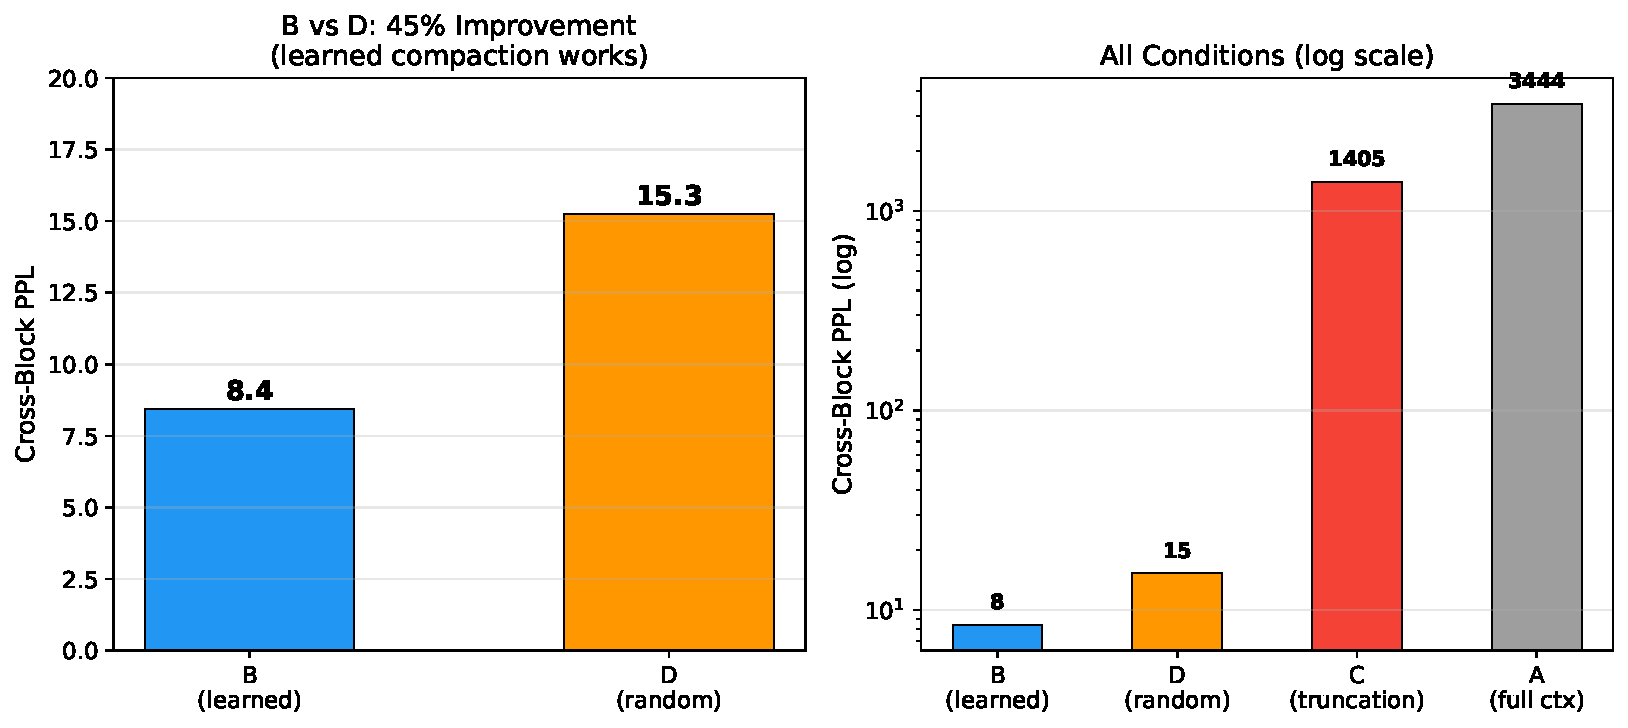
\includegraphics[width=\textwidth]{fig3_comparison.pdf}
\caption{\textbf{Left}: B vs D cross-block PPL (linear scale). B achieves 45\% lower
perplexity, demonstrating learned compact\_kv carries useful information.
\textbf{Right}: All conditions on log scale. A and C have extremely high cross-block PPL
because they were not trained with the blockwise mechanism.}
\end{figure}

\section{Bug Discovery \& Fix}

A critical label alignment bug was discovered during Phase 2a: \texttt{labels[j] = token\_ids[j]}
(identity) instead of \texttt{token\_ids[j+1]} (next-token). This caused the model to predict
the current token from its own embedding — trivially solvable (PPL $\approx$ 1.0) and masking
the compaction signal entirely. The bug was caught by an adversarial subagent when B $\approx$ D
in the initial (buggy) run. After fixing, all results shown above use correct labels.

\section{Scale-Up Experiments (In Progress)}

Six conditions are currently training across 6 NERSC Perlmutter nodes (24$\times$ A100-80GB):

\begin{table}[H]
\centering
\begin{tabular}{llccl}
\toprule
Condition & Node & GPUs & batch\_total & Status \\
\midrule
B ($K$=2, $P$=16) & nid008205 & 4 & 512 & Step $\sim$50/600 \\
D (random kv) & nid008268 & 4 & 512 & Step $\sim$50/600 \\
E (no compact\_kv) & nid008297 & 4 & 512 & Step $\sim$50/600 \\
B ($K$=4) & nid008304 & 4 & 512 & Step $\sim$50/600 \\
B ($P$=32) & nid008448 & 4 & 512 & Step $\sim$50/600 \\
A (full context) & nid008480 & 4 & 512 & Step $<$50/600 \\
\bottomrule
\end{tabular}
\caption{Scale-up runs. Each uses 4-GPU DDP with manual gradient all-reduce
(no DDP wrapper due to BPTT backward complexity). lr=$10^{-4}$, 50K examples/dataset.
Estimated completion: $\sim$27 hours per blockwise condition.}
\end{table}

Key hypotheses being tested:
\begin{itemize}
    \item \textbf{B vs E}: Does compact\_kv help vs. no cross-block information? (fairest baseline)
    \item \textbf{B vs D}: Does the B-vs-D gap widen with more training? (expected from Phase 2a trend)
    \item \textbf{B $K$=4 vs $K$=2}: Does deeper BPTT help? (Phase 1 found $K$=4 best)
    \item \textbf{B $P$=32 vs $P$=16}: Do more compaction tokens help? (Phase 1 showed monotonic improvement)
\end{itemize}

\section{Conclusion}

Phase 2a provides strong proof-of-concept evidence that KV Self-Compaction scales to
0.6B-parameter models. The 45\% improvement of learned compact\_kv over random noise,
combined with the mechanistic evidence of attention bias divergence, demonstrates that
the compaction tokens learn to carry useful cross-block information. Scale-up experiments
are underway to confirm these results with more data and training, and to explore the
$K$ and $P$ hyperparameter space.

\end{document}
